\chapter{Projektbeskrivelse}


\section{Projektgennemførelse}
Ud fra den givne projektformulering og tilgang til emnet er der udformet en tidsplan, som indeholder de overordnede deadlines for review og tests givet fra AU.
\begin{figure}[H]
	\centering
	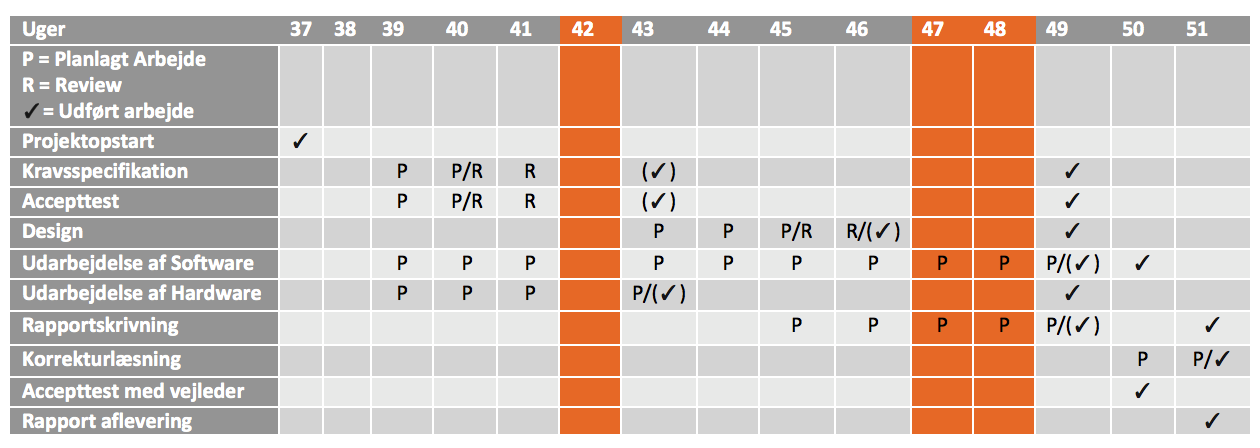
\includegraphics[width=1\textwidth]{Figurer/Snip20151210_74.png}
	\caption{Overordnet tidsplan}
\end{figure}
Udviklingsprocessen "Scrum" er blandt andet blevet brugt til at nedbryde opgaven i delelementer, hvor de vigtigste delopgaver er prioriteret først. Via Scrum inddeles arbejdet i sprints, hvilket tidsplanen ligeledes er blevet. Sprints er forskellige faser, som eksempelvis projektopstart, kravspecifikation, accepttest, design osv.\\\\
I tidsplanen er der markeret et P for det planlagte arbejde, hvor reviews er markeret med bogstavet R. Derudover er der markeret flueben i tidsplanen for udført arbejde. Flueben i parentes repræsenterer, hvornår arbejdet skulle have været færdigt, men ikke blev det. Uge 42 er markeret med orange farve, da der var efterårsferie, og her var der heller ikke planlagt arbejde. Uge 47 og 48 er også markeret med orange farve og bogstavet P, da der i denne periode har været planlagt arbejde. Dette arbejde er dog ikke blevet udført grundet eksamenslæsning og eksamen.
\\\\
\\\\
\\\\
\subsection{Deadlines}
Der er fra projektets start blevet stillet deadlines til forskellige dele af projektet.

\begin{longtabu} to \linewidth{@{}l X[j]@{}}
	Dato &    Deadlines \\[-1ex]
	\midrule
	02.10.2015		&	Aflevering af kravspecifikation og accepttest til review-gruppen \\[-1ex]
	09.10.2015			&	Review af kravspecifikation og accepttest færdiggjort med review-gruppen\\[-1ex]
	06.11.2015		&	Aflevering af design til review-gruppen \\[-1ex]	
	13.11.2015		&	Review af design færdiggjort med review-gruppen \\[-1ex] 
	11.12.2015		&	Accepttest med vejleder\\[-1ex]
	16.12.2015		&	Aflevering af projekt\\[-1ex]
	\caption{Deadlines}
\end{longtabu}
De første to deadlines i Tabel 6.1 har omhandlet kravspecifikation og accepttesten, hvor kravspecifikation er blevet udarbejdet først, efterfulgt af accepttesten. Derudover har der været deadlines til design, samt accepttest med vejleder og projektaflevering. 

\subsection{Mødestruktur}
Der er blevet fastlagt mødestruktur ved projektets start, hvor alle gruppens medlemmer har udarbejdet en samarbejdsaftale. Et ugentligt møde med vejleder efterfulgt af gruppemøde er blevet afholdt hver onsdag. Derudover er der blevet holdt gruppearbejde/gruppemøde efter behov. Hvert møde er blevet indledt med en opsamling af projektet og en dagsorden for mødet. Til kommunikation omkring møder, er der benyttet Facebook og en fælles kalender over iCloud.  \\\\ Der er blevet ført logbog for samtlige møder med vejleder, samt logbog ved møder gruppemedlemmerne imellem.

\subsection{ASE-modellen}
Projektets udviklingsproces har taget udgangspunkt i ASE-modellen, som ses på nedenstående Figur 6.2. Denne afspejles desuden også i den overordnede tidsplan (Figur 6.1.). 
\begin{figure}[H]
	\centering
	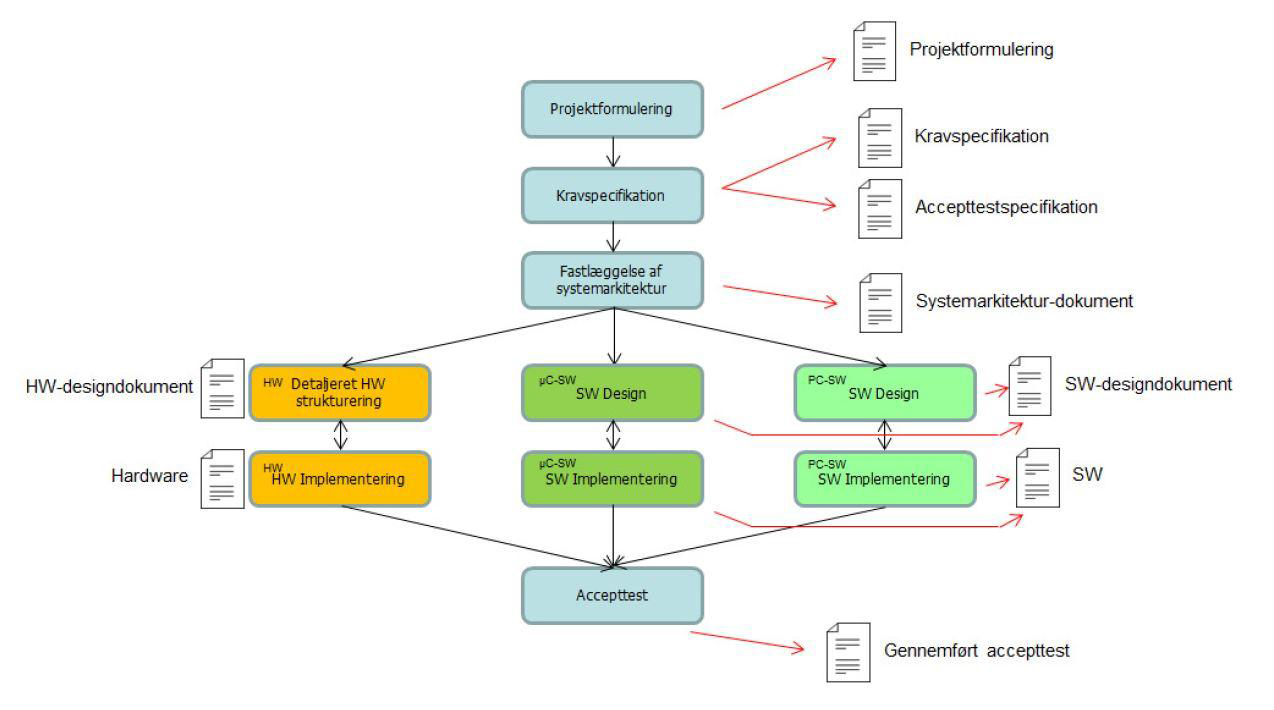
\includegraphics[width=1\textwidth]{Figurer/asemodel}
	\caption{Udviklingsmodel: ASE-model \protect\cite[s. 6]{Vejledning}}
\end{figure}
ASE-modellen er en udviklingsmodel, der tager udgangspunkt i Use Cases, som defineres i kravspecifikationen i starten af projektarbejdet. ASE-modellen er inspireret af vandfaldsmodellen, hvor projektarbejdet opdeles i faser. Der fastlægges en opgaveformulering, kravspecifikation og systemarkitektur, for derefter at designe, implementere og teste de enkelte moduler i iterationer. Ud fra projektformuleringen specificeres kravspecifikationen som en række Use Cases, der beskriver de forskellige aktørers interaktion med systemet. Dette giver et overblik over, hvilke krav, der stilles til systemets funktionalitet. Ud fra kravspecifikationen bliver systemets accepttest udarbejdet. Efter kravspecifikationen er fastlagt, udarbejdes systemarkitekturen. Ud fra systemarkitekturen designes systemet ved at nedbryde det efter funktionalitet, som kan bindes til både software og hardware. \\\\
De første step i udviklingen af projektet ifølge ASE-modellen, er blevet udarbejdet af alle gruppens medlemmer. Alle har bidraget til projektformuleringen, kravspecifikationen og accepttesten. I begyndelsen var der primært fokus på at få dette færdiggjort, men der blev allerede her arbejdet på komponentværdier og udkast til hardwaren. I starten af projektarbejdet var det udtænkt, at alle gruppens medlemmer skulle arbejde med alle områder i projektet. Dette kunne ikke udføres rent tidsmæssigt, og derfor var en opdeling af arbejdsopgaver i mindre grupper nødvendig. Det blev delt op i software- og hardwarehold, dog var en del af hardwaren allerede beregnet og implementeret, da denne opdeling fandt sted. Tilbage af hardwaredelen var at lodde det på et veroboard og derefter teste det.\\\\

\subsection{V-modellen}
V-modellen er en udviklingsmodel opdelt i forskellige faser, der beskriver udviklingsfaserne og testfaserne i projektet sideløbende. Denne model er blevet benyttet sideløbende med ASE-modellen, og fungerer således, at specifikationen af tests foregår sideløbende med udviklingen af selve systemet. Hver fase skal færdiggøres inden næste fase påbegyndes, hvilket også var tiltænkt i projektet. Dette blev dog ikke helt opfyldt i projektet, da der ofte blev rettet i tidligere faser, selvom de reelt skulle have været færdiggjort.
\begin{figure}[H]
	\centering
	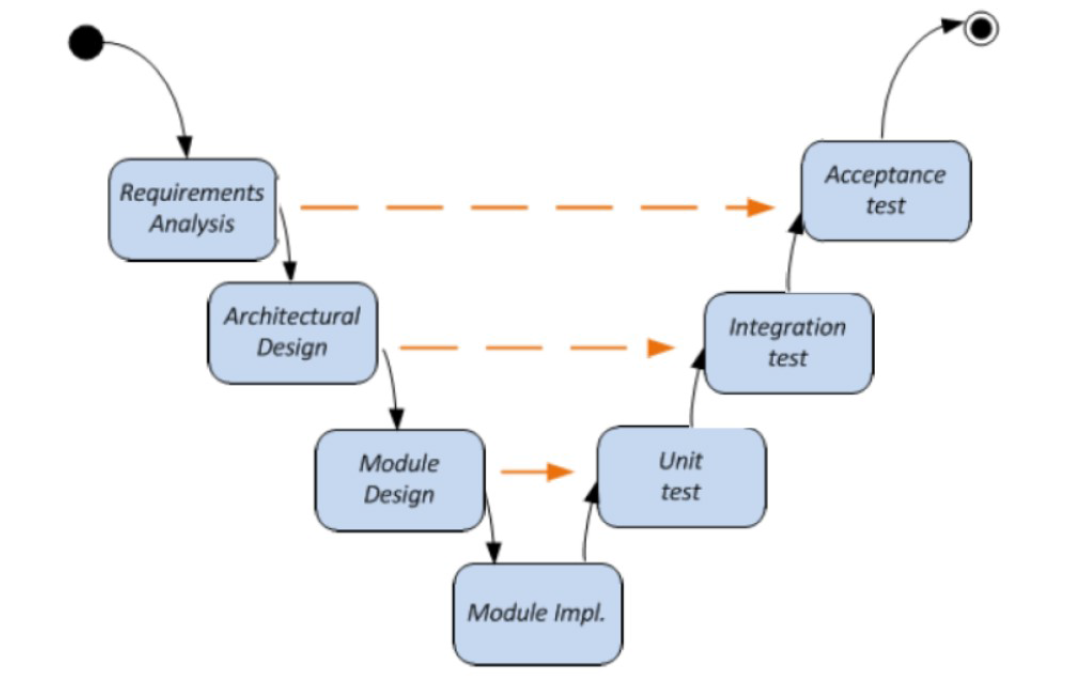
\includegraphics[width=1\textwidth]{Figurer/vmodel}
	\caption{V-modellen, \protect\cite[s. 4]{Vejledning}, \protect\cite{ISE}}
\end{figure}
På ovenstående figur ses V-modellen, hvor den første fase er udviklingen af kravspecifikationen. Hertil udvikles en tilhørende accepttest, som gør det muligt, at tjekke om systemet opfylder de stillede krav. Næste fase er systemarkitekturen, hvor der ligeledes udvikles en tilhørende test. Testen skal undersøge integrationen mellem de implementerede moduler. De to sidste faser er design og implementering, som der udføres løbende tests af. 

\subsection{Vandfaldsmodellen}
Vandfaldsmodellen er en model, der ofte benyttes for udviklingen af software. Udviklingen af software foregår på den måde, at en ny fase af modulen først påbegyndes, når den foranliggende fase er færdiggjort, som kan ses i Figur 6.4. nedenfor. 
\begin{figure}[H]
	\centering
	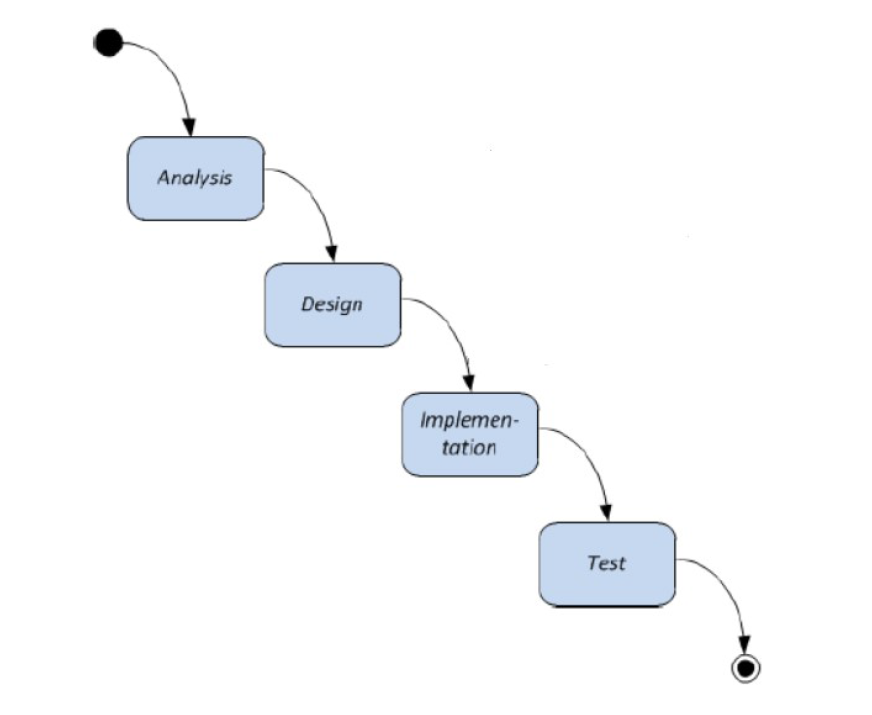
\includegraphics[width=0.8\textwidth]{Figurer/vfmodel}
	\caption{Vandfaldsmodellen, \protect\cite{ISE}}
\end{figure}
De tre udviklingsmodeller hænger alle sammen på den måde, at der arbejdes i kronologisk logisk rækkefølge. De har suppleret hinanden alle tre, hvor ASE-modellen har skabt det overordnede overblik. Vandfaldsmodellen er den udviklingsproces, som der er blevet arbejdet efter i alle projektets facetter. V-modellen har sikret, at de nødvendige tests af systemet og de enkelte moduler har fundet sted. 



\section{Metode}
Dette afsnit har til formål at beskrive, hvilke metoder samt arbejdsredskaber, der er blevet benyttet til udarbejdelsen af software, hardware, rapport og dokumentation for projektet. 
\\\\
Der er blevet anvendt metoder og viden fra forskellige kurser over 1.- 2.- og 3.semester. I kurset ST3KVI er der blevet benyttet viden om transducerprincippet samt generelt om blodtryksmåling, hvor der er i dette projekt fokuseres på den invasive blodtryksmåling. Fra kurserne ST2ITS2 og ST3ITS3 har viden om databasestruktur, principperne om trelagsmodellen og observer \& strategy pattern været grundlaget for opbygningen af softwaren. Et krav til projektet var, at der skulle kunne aktiveres og deaktiveres et digitalt filter. Til at designe dette filter blev der anvendt viden fra kurset E3DSB. Kurset ST1SUN1 har bidraget med viden om blodtryk og den anatomiske opbygning af hjertet. Til beregning af komponentværdier, design og implementering af hardwaren, er der blevet benyttet metoder og viden fra kurset E2ASB. Principperne om design diagrammer fra kurset I2ISE har bidraget til designafsnittet for hardware og software i dokumentationen. Alle kurserne har tilsammen været nødvendige for, at kunne udvikle et blodtryksmålesystem.
\\\\
Ved hjælp af SysML, er software- og hardwaredesign blevet specificeret. Det er en metode, der anvender forskellige diagrammer til at beskrive opbygning og kommunikation for både software og hardware. Selve systemet vil også blive beskrevet ved brug af SysML. Hensigten er at give læseren det store overblik over, hvilke aktører, der interagerer med systemet, samt hvilken funktionalitet, der tillægges systemet.
\\ \\
Softwaren er også beskrevet ved hjælp af UML - helt specifikt ved et UML klassediagram. Klassediagrammet viser, hvilke klasser og metoder al softwaren består af, samt hvordan systemet er bygget op efter trelagsmodellen.
\\\\
For at forstå det grundlæggende om blodtryk og blodtryksmåling, er der blevet anvendt en redegørende metode, hvor der er blevet indsamlet viden gennem læsning af hjemmesider og sundheds- og tekniskfaglige bøger. Ud fra den viden har det været muligt, at redegøre for principperne, samt at analysere de resultater systemet har givet.
\\\\
Efter hardwarens funktionalitet var bestemt, blev den matematiske metode benyttet til at beregne de nødvendige komponentværdier, der skulle til for at realisere den ønskede hardware.

\subsubsection{Arbejdsredskaber} 
Af benyttede arbejdsredskaber er der først og fremmest brugt en fælles arbejdsplatform, GitHub. GitHub er en online platform, hvor der er mulighed for at foretage ændringer samtidigt, og gemme i en fælles mappe. Yderligere er der mulighed for en detaljeret versionshistorik.\\
Alle SysML- og UML-diagrammer er udarbejdet i programmet Visio. Koden er skrevet i sproget C\# i programmet Visual Studio. Visual Studio spiller også sammen med programmet WaveForms Generator, i forbindelse med simulering af blodtrykssignalet. Selve rapporten, mødereferater, logbog og dokumentationen er udformet i tekstprogrammet LaTeX. MatLab, som er et matematik- og signalbehandlingsprogram, er blevet benyttet til at udarbejdelse af hardwaren. Yderligere er Facebook og en fælles iCloud kalender blevet brugt til mødeindkaldelse og generel kommunikation.



\section{Specifikation og analyse}
Dette afsnit har til formål at beskrive de løsninger, der benyttes i forhold til de valgte hardware og software specifikationer. 

\subsection{Hardware}
Den udviklede hardware, som omtales Signalbehandlingsblok, består af en Forstærker og et Filter. Forstærkeren har til opgave at forstærke det elektriske signal, som Tryktransduceren har transformeret ud fra en given trykændring. Filterets opgave er at filtrere unødige frekvenser fra for, at få det mest optimale signal.
\\\\
\subsubsection{Tryktransducer}
Eksitationsspændingen for Forstærkeren og Filteret leveres af to 9 V's batterier. Der er valgt, at sætte en 5 V's regulator i forbindelse med Tryktransduceren for at sikre, at strømmen gennem Wheatstone broen ikke bliver for stor. En for stor strøm kan give anledning til, at Wheatstone broen vil drive og eventuelt brande de fire strain gauges af.\\
For at kunne beregne de tilstrækkelige komponentværdier for Forstærkeren og Filteret bestemmes en maksimal trykændring, den udviklede hardware skal kunne klare. Den maksimale trykændring for dette system er sat til at være i intervallet 0-300 mmHg. Da det er blodtryk, systemet skal kunne monitorere, er denne trykændring tilstrækkelig, da man ikke forventer, at et blodtryk vil komme over 300 mmHg.

\subsubsection{Forstærker}
Tryktransduceren vil transformere et tryk på 300 mmHg om til 7,5 mV - se Projektdokumentationen under grænseflader for udregningen (2.2). Denne spænding er forholdsvis lille, og vil ikke udnytte DAQ'ens måleområde optimalt, som er valgt til +/- 5 V. Så for at få den bedste konvertering af det analoge signal til det digitale signal, skal spændingen forstærkes op til 5 V. 
\\\\
Til dette benyttes den ikke-inverterende operationsforstærker, INA114 samt et potentiometer, der fungere som gain-modstanden. Gain-modstanden er en variabel modstand, der kan variere i forhold til, hvilken forstærkning, der ønskes. Udregningen for forstærkningen ses i Projektdokumentationen under Hardware arkitektur (2.3) under ligningerne (2.4) og (2.5). Udregningen for gain-modstanden kan ses i Projektdokumentationen under HW implementering og test (3) under ligning (3.3).     

\subsubsection{Filteret}
Det forstærkerede analoge signal skal videre filteres før det konventeres til det digitale signal. De relevante frekvenser, der udgør en blodtryksmåling ligger mellem 0-50 Hz \cite[s. 10]{Billed for invasiv blodtryksmaling} . Derfor ønskes alle frekvenser over 50 Hz dæmpet.
\\\\
Til dette designes et Sallen Key anden ordens lavpasfilter med unity gain, hvor cutofffrekvensen er 50 Hz. Udregningerne for kompontværdierne til denne realisering, se HW implementering og test (3) i Projektdokumentationen under Filterblok (3.2).

\subsection{Software} 
\subsubsection{Arkitektur}
Beslutningen om at anvende trelagsmodellen blev overvejende taget på baggrund af de krav der var stillet til projektet om, at der skulle ske en dataopsamling, databehandling og visualisering. De 3 lag repræsenterer hver især disse opgaver. 
For at overskueliggøre og effektivisere softwaren var en vigtig overvejelse navngivning af klasser og metoder efter deres pågældende funktion. Dette skaber høj samhørighed, og lav kobling klasserne imellem.\\
Data-laget er et eksempel herpå, med en opdeling i 3 klasser, med hver deres specifikke funktion(DataHent, DataGem, DAQ). På denne måde er fejlfinding overskueligt, da fejlen sker i en indkapslet funktion.

\subsubsection{Dataindhentning}
I overvejelserne omkring udskrivning af målt blodtryk til graf i monitor vinduet, var en prioritet at signalet blev udskrevet rettidigt, altså med en minimal forsinkelse fra at målingen var foretaget af den fysiske DAQ. I den forbindelse var det muligt enten at requeste data fra logiklaget jf. 3.lags modellen, eller at anvende subscriber/publisher pattern, med DAQ klassen som publisher. Ved den første metode, ville behandlingen af måledata være styret eksternt fra hvor data blev produceret, altså fra logik laget. Med den anden mulighed ville databehandlingen være styret af den fysiske DAQ. Dette var at foretrække, da data ville blive behandlet som det blev produceret; altså mest rettidigt.


\section{Arkitektur}
I følgende afsnit beskrives systemarkitekturen for blodtryksmålesystemet. Systemarkitekturen fungerer som en udviklingsramme for videreudviklingen af design og implementering. Her bliver systemets funktionalitet nedbrudt til overordnede moduler. Gennem dette afsnit ønskes der at skabe et overordnet overblik over systemet. Der benyttes diagrammer med tilhørende beskrivelser til at specificere og klarlægge systemkrav.

\subsection{Hardwarearkitektur}
Systemets hardware kan illustreres i et bdd og ibd, der beskriver det overordnede system og hvordan de forskellige hardwareblokke interagerer med hinanden. På Figur 6.5 ses bdd, der viser blodtryksmålesystemet bestående af fire hardwareblokke: Tryktransducer, Signalbehandling, DAQ og Computer. Hertil ses også hvilke porte, blokkene består af.
\begin{figure}[H]
	\centering
	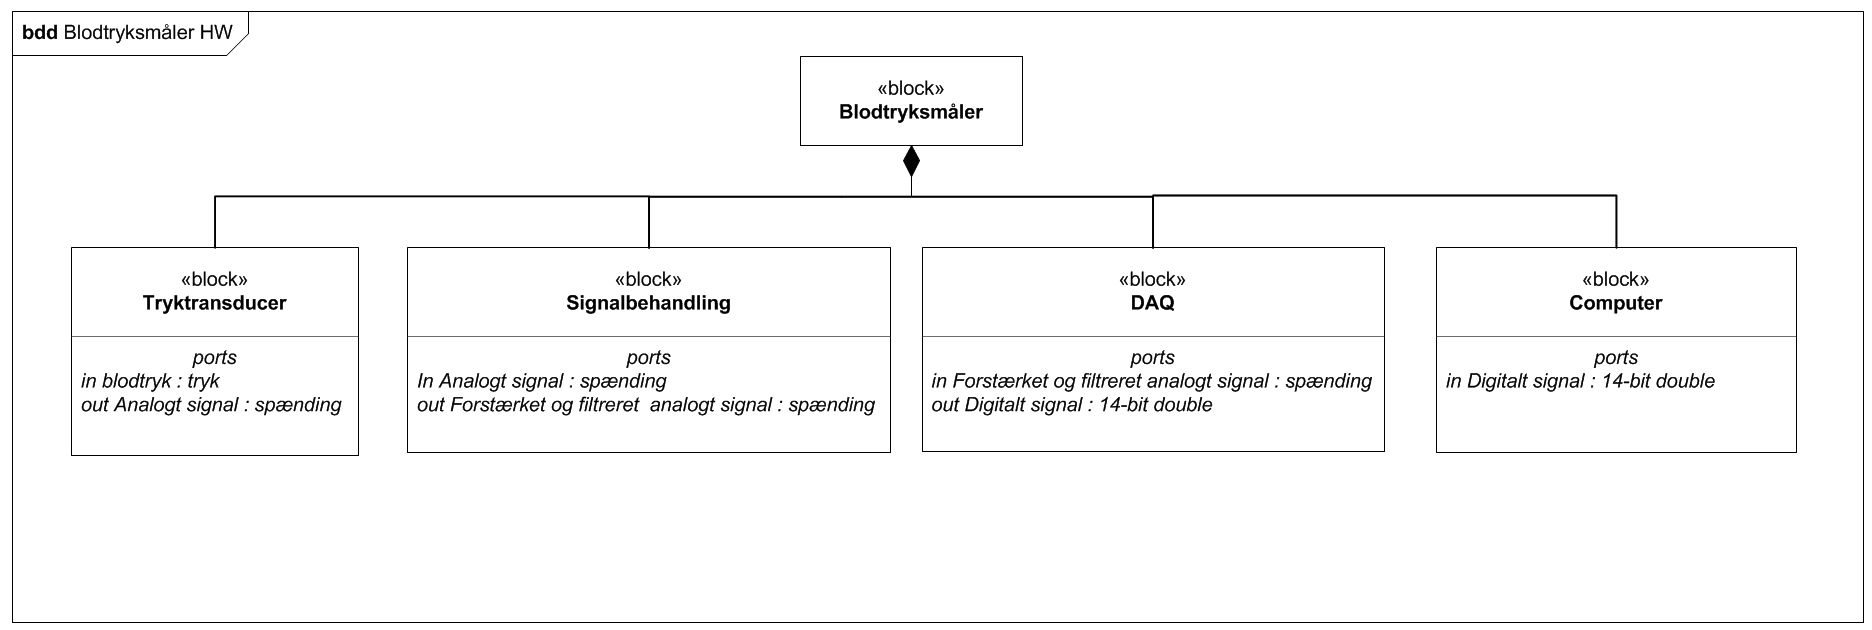
\includegraphics[width=1\textwidth]{Figurer/Snip20151209_70}
	\caption{bdd af blodtrykmålesystemet}
\end{figure}
Tryktransduceren registrerer en fysisk størrelse i form af en trykændring. Dennes opgave er at transformere det fysiske tryk til en elektrisk spænding, som derefter viderebehandles. Viderebehandlingen foregår i Signalbehandlingsblokken, som består af to dele: en Forstærker og et Filter. Her bliver det elektriske signal forstærket og filtreret således, at det er klar til at blive konverteret i DAQ’en fra et analogt til et digitalt signal. Computeren indeholder software til systemet, som kan vise det digitale signal grafisk, samt kalibrere, nulpunktjustere og gemme målinger. Derudover kan software aktivere og deaktivere Filteret.  
Bdd benyttes til at definere relationen mellem de forskellige blokke, som i dette tilfælde er en komposition. 
\begin{figure}[H]
	\centering
	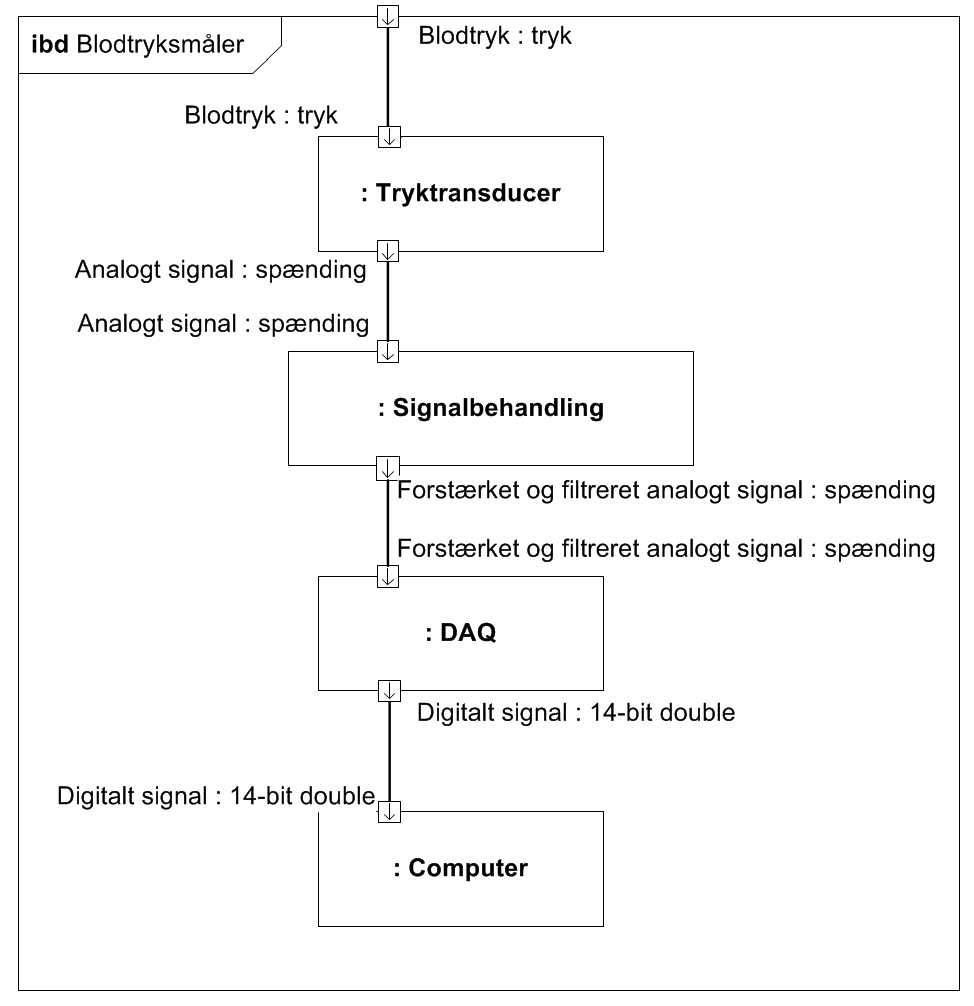
\includegraphics[width=0.8\textwidth]{Figurer/Snip20151209_72}
	\caption{ibd af blodtrykmålesystemet}
\end{figure}
På Figur 6.6 ses ibd for systemet, der viser signalets behandling gennem systemet. Signalet transformeres fra et målt fysisk tryk til et digitalt signal, som software kan viderebehandle og vise grafisk. For yderligere informationer om grænseflader (2.2) henvises der til Projektdokumentationen under design.

 
\subsection{Softwarearkitektur}
Systemets softwaredesign beskrives i dette afsnit via domænemodellen, som ses på Figur 6.7. Domænemodellen er skabt på baggrund af kravspecifikationens seks Use Cases, og viser et samlet overblik over systemet. 
\begin{figure}[H]
	\centering
	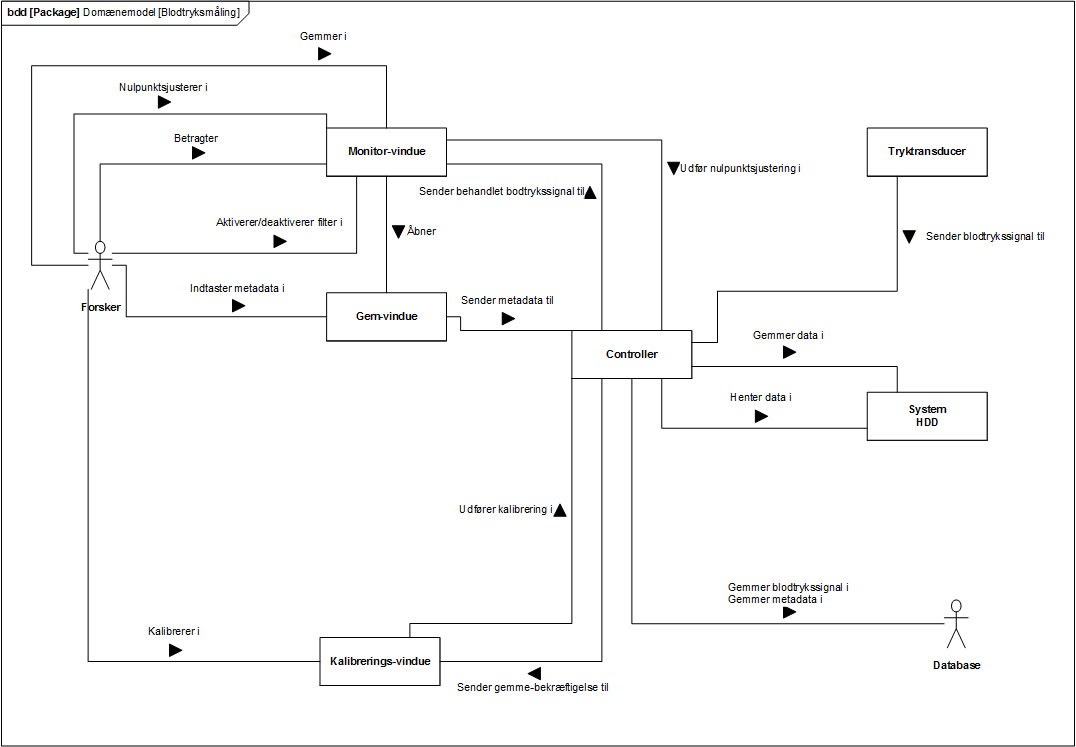
\includegraphics[width=1\textwidth]{Figurer/dm}
	\caption{Domænemodel af blodtrykmålesystemet}
\end{figure}
I domænemodellen ses interaktionen mellem de konceptuelle klasser og aktører. Controlleren udfører kommandoer og sørger for, at systemet fungerer optimalt. Funktionaliteten af den enkelte kommando kan variere fra Use Case til Use Case. Domænemodellen viser desuden Forskerens interaktion med systemet. Forsker udfører en handling, der medfører igangsættelse af en række processer i systemet. 
For yderligere information om forløbene i de seks Use Cases (2.4.2) henvises der til Projektdokumentationen under design. 


\section{Design, implementering og test}
I følgende afsnit vil design- og implementeringsprocessen for den udviklede hardware og software beskrives. Der vil være en beskrivelse af, hvordan de valgte løsninger er blevet testet. 

\subsection{Hardware}
Under afsnittet Specifikation og analyse (6.3.1) står specifikationer for Signalbehandlingsblokken beskrevet. Signalbehandlingsblokken består af en Forstærker og et Filter. Kommunikationen internt for Signalbehandlingsblokken, samt kommunikationen ud ad til, ses i ibd'et for Signalbehandlingsblokken i Figur 6.8 nedenfor.  

\begin{figure}[H]
	\centering
	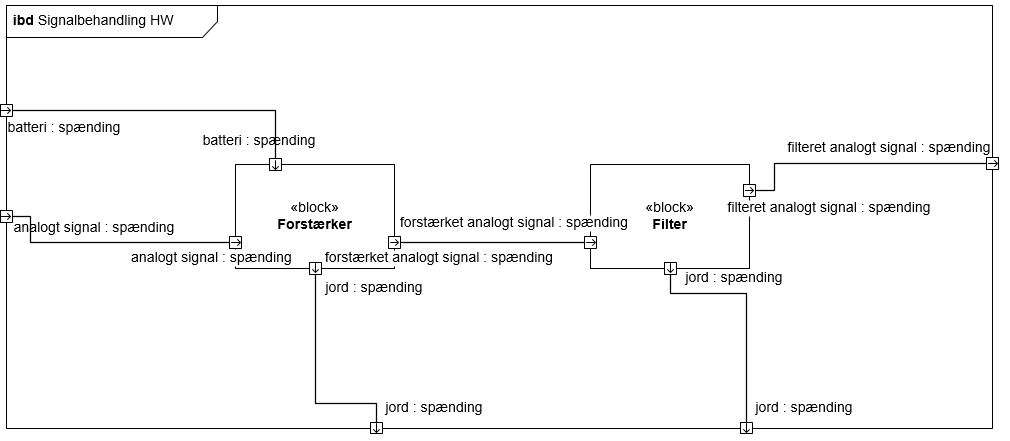
\includegraphics[width=1\textwidth]{Figurer/5}
	\caption{idb for Signalbehandlingsblokken}
\end{figure}

Til realisering af specifikationen for Forstærkeren er der blevet beregnet den ønskede forstærkning og gain-modstand, så et tryk på 300 mmHg forstærkes op til 5 V.\\
Udregningen for forstærkningen ses i Projektdokumentationen under Hardware arkitektur (2.3) under ligningerne (2.4) og (2.5). Udregningen for gain-modstanden kan ses i Projektdokumentationen under HW implementering og test (3) under ligning (3.3).  
\\\\
Til realisering af specifikationen for Filteret er der blevet beregnet de forskellige komponentværdier, så filteret får en cutoff frekvens ved 50 Hz.\\
Udregninger for komponentværdierne, ses under HW implementering og test (3) i Projektdokumentationen under Filterblok (3.2). 
\\\\ 
Signalbehandlingsblokken blev i starten af projektet implementeret på et fumlebræt. På Figur 6.9 ses denne opstillingen. 

\begin{figure}[H]
	\centering
	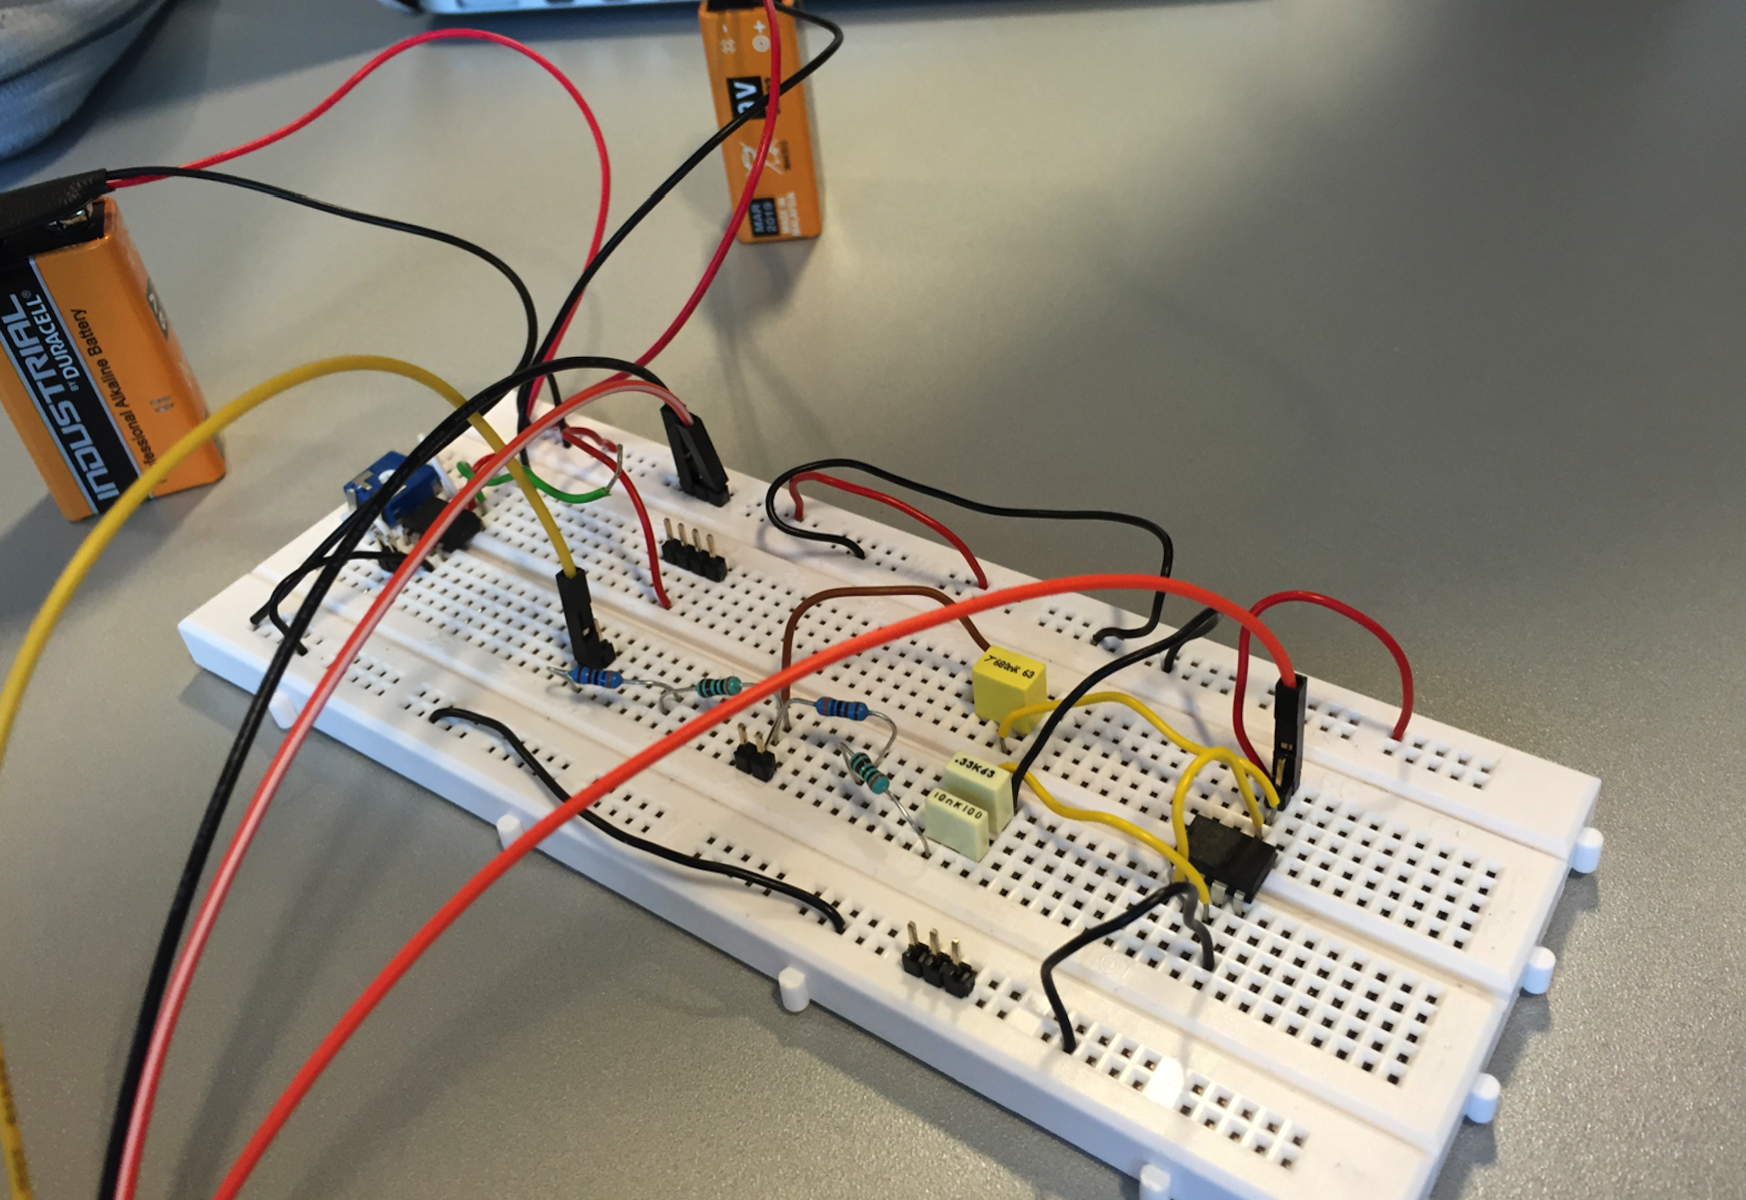
\includegraphics[width=0.7\textwidth]{Figurer/Snip20151213_83}
	\caption{Signalbehandlingsblokken implementeret på et fulmebræt}
\end{figure} 

Senere i implementeringsprocessen blevet Signalbehandlingsblokken implementeret på et veroboard. Dette blev valgt grundet bedre stabilitet og udseende. På Figur 6.10 ses veroboardet. Det var også tiltænkt, at Signalbehandlingsblokken skulle have været implementeret på en printplade, hvor forbindelsen mellem komponenterne er lavet på forhånd. Printpladens design skulle laves digitalt - først i programmet Multisim og videre i programmet Ultiboard. Dette blev ikke realiseret på grund af mangel på tid.

\begin{figure}[H]
	\centering
	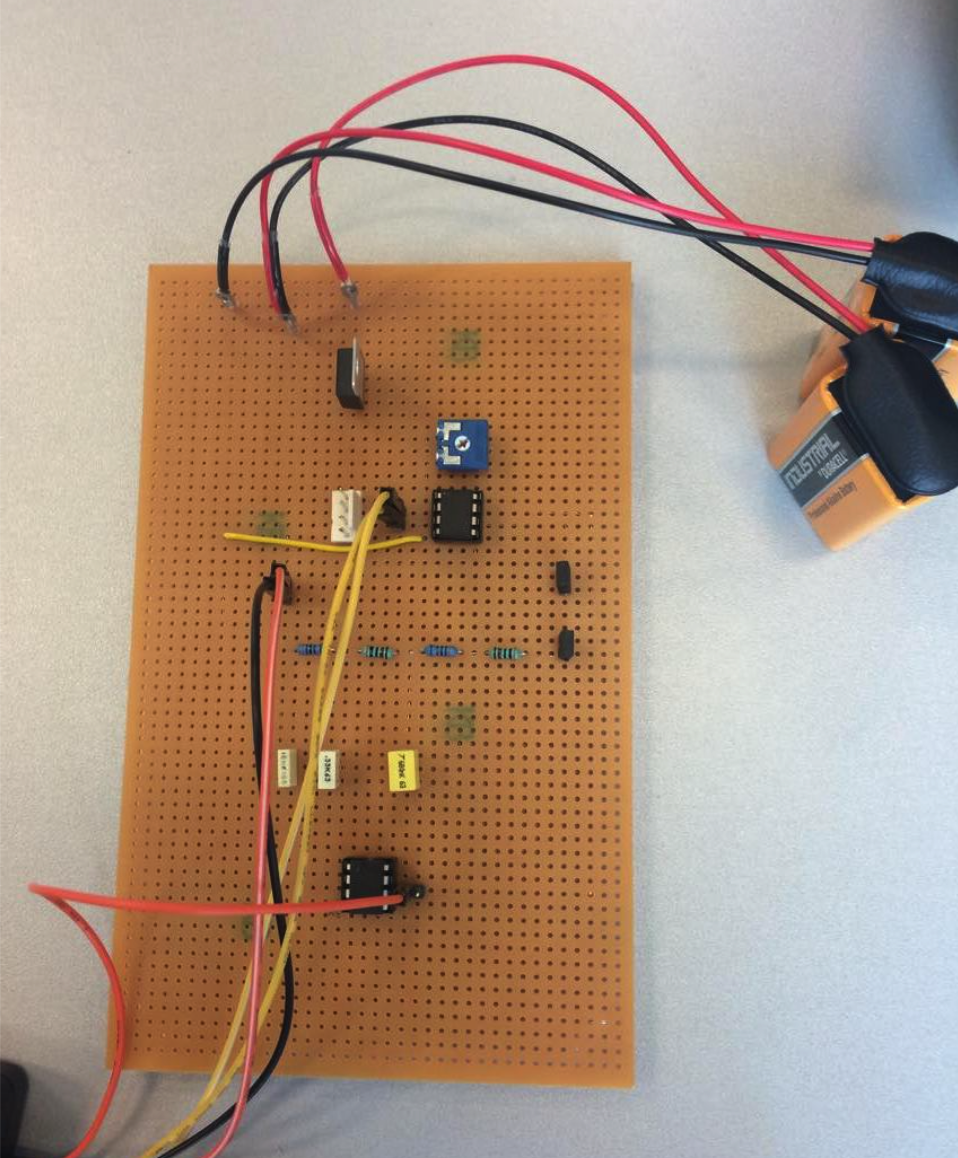
\includegraphics[width=0.6\textwidth]{Figurer/Snip20151207_46}
	\caption{Signalbehandlingsblokken implementeret på et veroboard}
\end{figure}

Signalbehandlingsblokken er blevet testet via Analog Discovery \& Waveforms. Først blev der lavet unit test, hvor Forstærkeren og Filteret blev testet hver for sig, og derefter blev der lavet en integrationtest, hvor Signalbehandlingsblokken blev testet som en enhed. 
\\\\
Specifikationen for forstærkeren er, at den skal forstærke en spænding på 7,5 mV, der svarer til et tryk på 300 mmHg, op til 5 V. \\
Signalgeneratoren leverer inputspændingen, hvor oscilloskopet måler outputspændingen. Inputspændingen kan via Waveforms bestemmes. Til denne unit test af Forstærkeren sættes inputspændingen til 7 mV. Reelt burde den sættes til 7,5 mV, men det er ikke muligt. \\
Den forventede outputspænding, ved en inputspænding på 7 mV, er 4,7 V - se Projektdokumentationen under Test af forstærkerblok (3.2.1) for udregningen, samt dokumentationen af denne test.
Resultatet af testen stemte overens med det forventede. 
\\\\
Specifikationen for filteret er, at den skal dæmpe frekvenser over 50 Hz. Denne specifikation realiseres via et anden ordens lavpasfilter. \\
Til denne unit test af Filteret sættes inputspændingen til 5 V. For at teste om det implementerede Filter har en cutoff frekvens ved 50 Hz ændres inputspændingens frekvenser. Der laves ialt tre tests. Først testes Filteret, hvor frekvensen er 1 Hz. Her forventes det, at outputspændingen er lig med inputspændingen. Derefter testes Filteret, hvor frekvensen er 50 Hz. Her forventes det, at outputspændingen er blevet dæmpet med 3 dB. Til sidst testes Filteret, hvor frekvensen er 500 Hz. Her forventes det, at outputspændingen er blevet dæmpet med 40 dB. I Projektdokumentationen under Test af filterblok (3.2.2) og i dokumentationen af denne unit test, ses de forventede outputspændinger ved de forskellige frekvenser.
Resultaterne af testen stemte overens med det forventede.  

    
 
 


 

\subsection{Software}
Softwaren er designet efter 3-lags modellen samt anvendelse af publisher/subscriber mønstret. \\
Dette er gjort i henhold til de givne krav til produktet, som er dataopsamling, databehandling og visualisering. 3-lagsmodellen sørger for at håndterer af disse opgaver sker i hvert sit lag. Det visuelle design er lavet så det assimilerer eksisterende blodtryksmonitorer. \\
Design af SW er konkretiseret i sekvensdiagrammer med konceptuelle klasser.
\\\\

Form-laget er implementeret med tre GUI vinduer: Monitor, Gem og Kalibrer.\\ 
Monitorvinduet udskriver blodtrykssignalet, giver bruger mulighed for at udføre nulpunktsjustering, og optage det viste signal. Gem vinduet fremviser det optagne signal, til revision før gemning på database. Kalibreringsvinduet giver bruger mulighed for kalibrering af systemet.\\ 
Logik laget er implementeret med en enkelt klasse, Beregninger, som udfører opgaver i specificerede metoder, såsom digital filtrering, kalibrering, nulpunktsjustering og behandling af rådata.\\
Datalaget er implementeret med klasser med specifikke opgaver, der sørger for lav kobling og høj samhørighed. Dataoverførslen af rådata sker jf. publisher/subscriber mønstret. \\
Implementeringens af software er beskrevet med sekvensdiagrammer med konkrete softwareklasser og metoder i projektdokumentationen.
\\\\

Softwaren er testet jf. use cases. Analog Discovery Waveform Generator er brugt som input til systemet, og resultater er kontrolleret med debugging af kode.


\section{Resultater og diskussion}
Accepttest blev den 9. december 2015 gennemført af vejleder Peter Johansen. Til denne test af blodtryksmålesystemet blev et blodtrykssignal fra PhysioNet simuleret ved hjælp af Analog Discovery \& Waveforms. Accepttesten blev gennemført uden nogen problemer og der kunne sættes checkmark ved alle funktionelle og ikke-funktionelle krav. 

\subsection{In Vitro hjertemodel}
Samme dag var det muligt, at teste blodtryksmålesystemet via en In Vitro hjertemodel. In Vitro betyder ”i glas”, hvilket er en betegnelse, man benytter, når man laver forskningsforsøg uden for den levende organisme. \\
Den benyttede In Vitro hjertemodel til testen af blodtryksmålesystemet genskaber hjertets venstre sides funktion. Trykket i modellen bliver skabt via stempelpumpen ViVitro SuperDup'r. Hjertets venstre side genskabes via et ventrikulær kammer, en artiel reservoir samt en aortarod. Mellem det ventrikulære kammer og det artielle reservoir sidder der en mekanisk hjerteklap, der efterligner funktionaliteten af mitralklappen. I aortaroden er aortaklappen også genskabt. Filmen ”Aortaklap” viser, hvordan aortaklappen fungere.\\
Via denne In Vitro hjertemodel kan hjertes venstre sides blod flow simuleres, hvilket gør det muligt at måle trykket efter aortaroden, hvilket kan sammenlignes med det artielle blodtryk.

\begin{figure}[H]
	\centering
	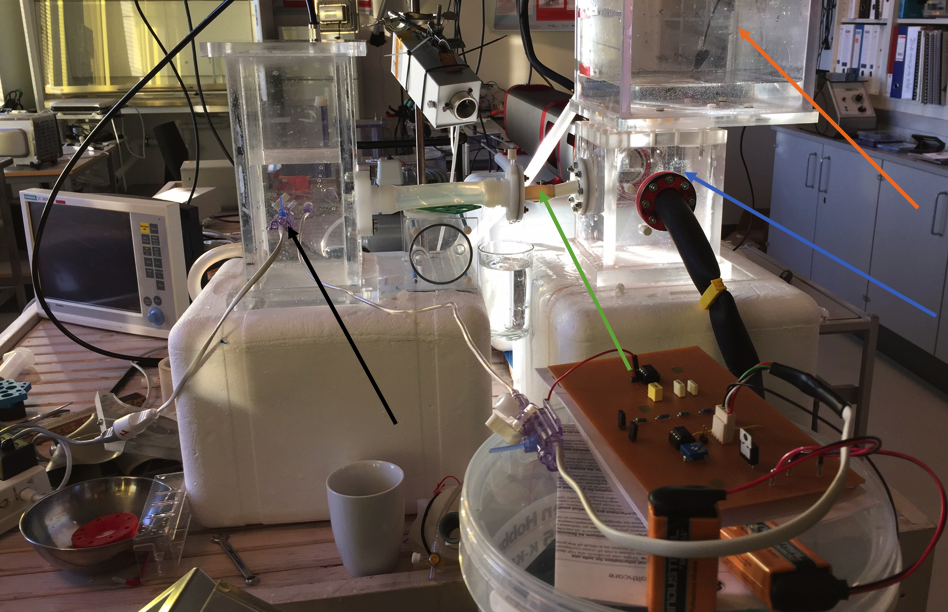
\includegraphics[width=1\textwidth]{Figurer/Snip20151214_98}
	\caption{Opstilling af In Vitro hjertemodel}
\end{figure}

På Figur 6.11 ses opstillingen for In Vitro hjertemodel. Den orange pil peger på den artielle reservoir, den blå pil peger på det ventrikulære kammer og den grønne pil peget på aortaroden. Tryktransduceren fastsættes der, hvor den sorte pil peger. På billedet ses, at der er fastsat to tryktransducer. Den ene er tilkoblet et monitoreringssystem fra Siemens, mens den anden er tilkoblet vores monitoreringssystem.
\\\\
Før målingen kan foretages skal vores monitoreringssystem kalibreres. Til dette benyttes en vandsøjle. På vandsøjlen er tre punkter markeret, hvor trykket i mmHg er kendt. Når monitoreringssystemet skal kalibreres, skal der bestemmes en kalibreringskonstant, som systemet skal korrigeres efter. \\
Der måles først en spænding ved eksempelvis 10 mmHg og derefter en spænding ved eksempelvis 50 mmHg. Kalibreringskonstanten beregnes ud fra følgende formel: 

\begin{equation}
	K_{konstant} = \frac{tryk_2 - tryk_1}{spænding_2 - spænding_1}
\end{equation}

Efter kalibreringen er foretaget kan målingen foretages. 
\\\\

Resultaterne af målingen ses på Figur 6.12 og Figur 6.13. Figur 6.12 viser resultatet af vores monitoreringssystem, mens Figur 6.13 viser resultatet af Simens’ monitoreringssystem. 

\begin{figure}[H]
	\centering
	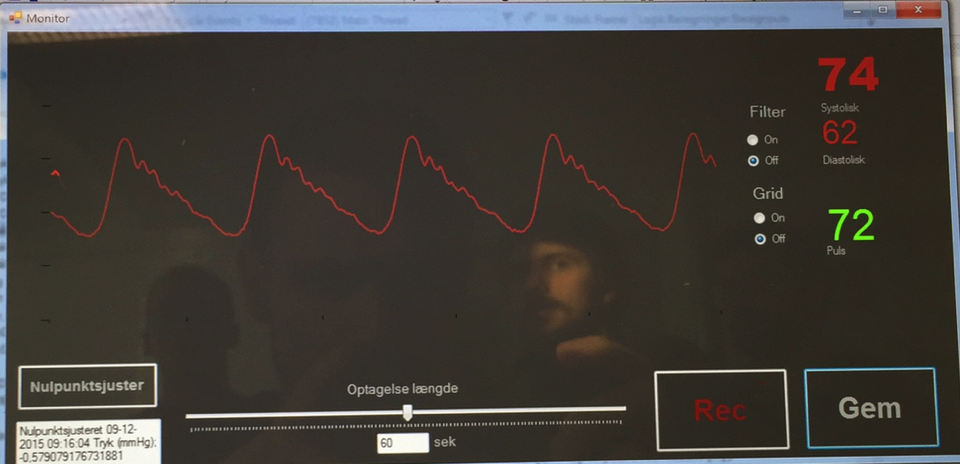
\includegraphics[width=1\textwidth]{Figurer/Snip20151214_99}
	\caption{Vores monitoreringssystem}
\end{figure}

\begin{figure}[H]
	\centering
	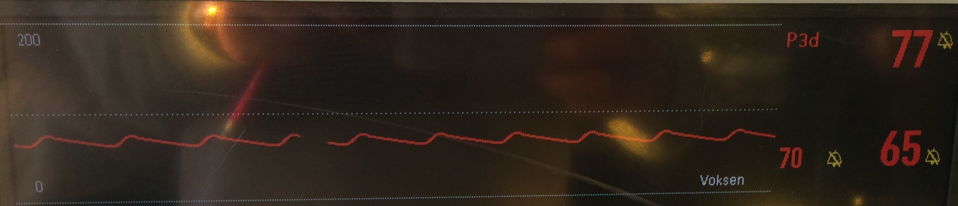
\includegraphics[width=1\textwidth]{Figurer/Snip20151214_100}
	\caption{Simens' monitoreringssystem}
\end{figure}

Der ses, at der er en lille forskel i værdier for de to monitoreringssystemer. Årsagen hertil kan være, at billederne ikke blev taget på nøjagtig samme tid, da dette ikke var muligt. Forskellen er dog så lille, at det accepteres. \\
Værdierne er heller ikke realistiske i forhold til det artielle blodtryk – systolen er meget lavere end det forventede. Årsagen til dette er opstillingen af In Vitro hjertemodel, hvor der var nogle problemer med pakningerne mellem det ventrikulære kammer og aortaroden samt at der var et lille hul i aortaroden, hvor vand ville sprøjte ud, hvis trykket fra stempelpumpen blev for stort.  Filmen ”Utæt pakning mellem ventrikulær kammer og aortaroden” i bilag viser dette.
\\\\

Ud fra denne test via In Vitro hjertemodel konkluderes det, at vores monitoreringssystem fungerer som ønsket, da de to monitoreringssystemer følges ad og viser tilnærmelsesvis samme værdier.

\subsection{Blodtryksmåling på en gris} 


Den 14. december 2015 var det muligt at teste blodtryksmålesystemet på en gris på Skejby Sygehus. Formålet med denne test, er at undersøge om blodtryksmålesystemet kan monitorerer et blodtryk, der kan sammenlignes med det menneskelige. \\
Målingen foregik på en gris, der blev benyttet til klinisk forskning. Selve operationen foregik samtidig med monitorering af blodtrykket. I en arterie tæt på sternum blev et kareter påsat, som gjorde det muligt at fastsætte tryktransduceren fra blodtryksmålesystemet. På Figur 6.14 ses resultaterne fra målingen. I det tidsrum, hvor vores blodtryksmålesystemet stod for monitoreringen, var det nødvendigt for lægerne at vide blodtryksværdierne. Disse kunne blodtryksmålesystemet levere og lægerne accepterede disse.

\begin{figure}[H]
	\centering
	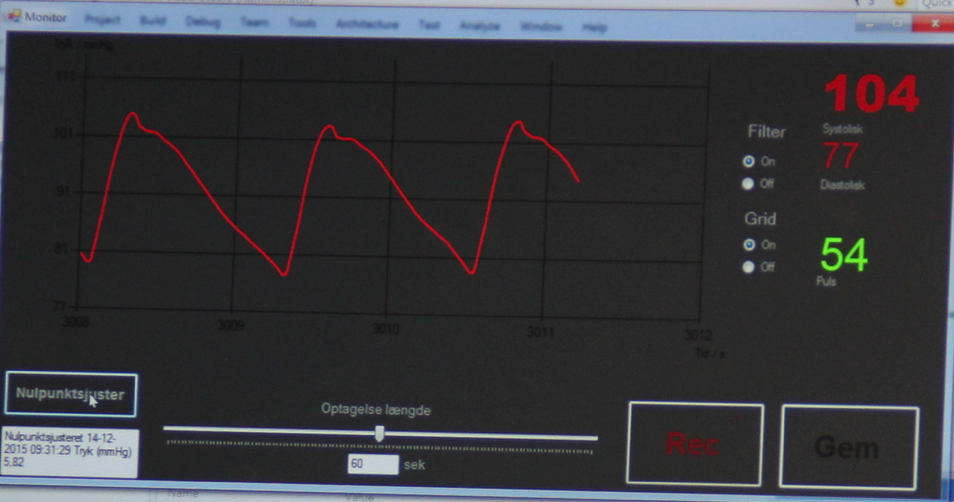
\includegraphics[width=1\textwidth]{Figurer/Snip20151214_101}
	\caption{Vores monitoreringssystem}
\end{figure}

Efter målingen blev sygehuset allerede implementeret system påsat. På Figur 6.15 ses dette monitoreringssystems resultater.

\begin{figure}[H]
	\centering
	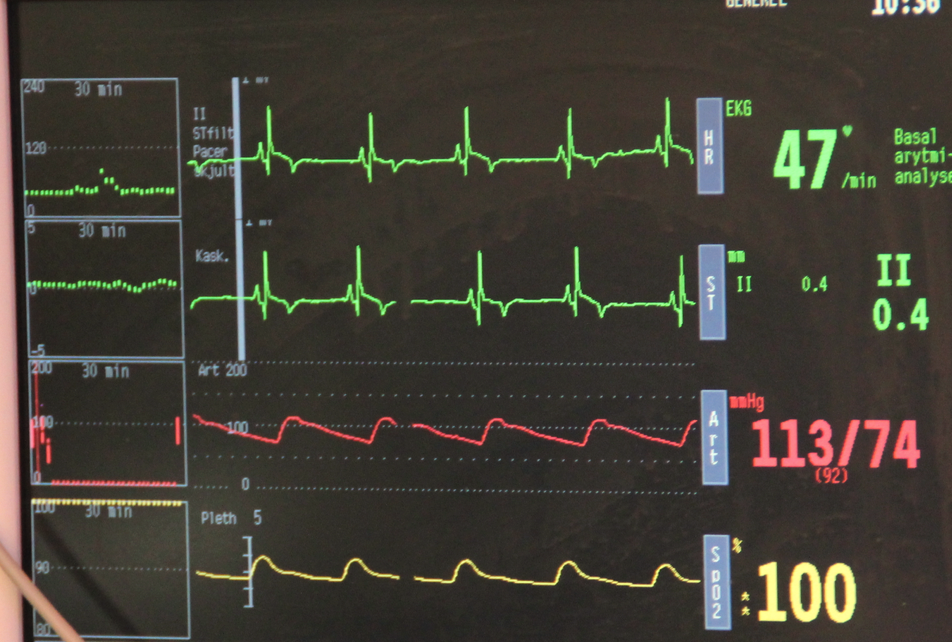
\includegraphics[width=1\textwidth]{Figurer/Snip20151214_102}
	\caption{Sygehusets monitoreringssystem}
\end{figure}


Igen ved denne test ses der en lille forskel i værdierne. Årsagen kan igen være, at billederne ikke blev taget på nøjagtig samme tid. Filmen ”Griseforsøg” i bilag viser blodtryksmålingen på grisen.
\\\\ 
Ud fra denne test af blodtryksmålesystemet konkluderes det, at vores monitoreringssystem fungere som ønsket, og kan monitorere reelle blodtryksværdier. 


\section{Opnåede erfaringer}
På baggrund af den generelle viden om hjertet, blodtrykket og de forskellige måletyper er der designet og udviklet et system til at måle blodtrykket invasivt. Med udgangspunkt i problemformuleringen og opsatte rammer er der arbejdet efter vandfaldsmetoden, hvor vi undervejs i udviklingsprocessen gennem løsninger og erfaringer har opnået bedre kendskab til det ønskede produkt. Vi har styrket vores tværfaglige kompetencer og formået at udvikle en teknisk løsning samt at benytte teori i praksis.\\\\
Et væsentligt fokusområde i udviklingen af blodtryksmålesystemet har været integreringen af hardware og software. I udarbejdelsen af hardware startede vi med at beregne komponentværdierne og derefter designe det elektriske kredsløb for at kunne opstille det på et fumlebræt. Herefter var hensigten at designe kredsløbet i Multisim, og derefter overføre det til printplade via Ultiboard. Dette blev ikke gennemført grundet tidspres. Derfor designede vi kredsløbet på et veroboard, hvor komponenterne og forbindelserne blev loddet. I selve processen med design af kredsløb opstod der problemer, da vi ved en fejl havde placeret de to kondensatorerne omvendt af hinanden, så de ikke stemte overens med teorien. \\\\
I udviklingen af det ønskede software har vi tildelt os ny viden i undervisningen i ITS3, men primært har softwaren været en viderebygning på erfaringer fra 2. semesterprojektet. Processen har været uden svære komplikationer, dog blev vi bevidste om et problem i forhold til udskrivning af samples. Da vi har målt med over 1000 samples i sekundet, erfarede vi at programmet ikke kunne udskrive dette. Dette løste vi ved i stedet kun at udskrive hvert 10. sample, hvilket dog indebar at signalet ikke blev lige så præcist. \\\\ 
Selve projektarbejdet har i høj grad været struktureret af faste møder og dagsordener. Derudover har der været en fælles opsamling på opgaver, der har været fordelt mellem gruppemedlemmerne. På denne måde har det været muligt for alle at have et overblik over de forskellige arbejdsopgaver. Denne strukturering af projektarbejdet har styrket vores færdigheder i projektstyring og tilrettelægning af arbejdsopgaver.


\section{Fremtidigt arbejde}
Gennem udviklingsforløbet af blodtryksmålesystemet, er der blevet arbejdet ud fra de retningslinjer og obligatoriske krav, der er blevet givet fra AU’s side. Første prioritet har været, at skabe et produkt der lever op til disse krav, men samtidig har der været fokus på at skabe det bedst mulige produkt for brugeren. Som resultat heraf, er der blevet implementeret udbyggende forbedringer i blodtryksmålesystemet i form af afbildning af systolisk/diastolisk blodtryk og puls med tal. \\
Yderligere forbedringer hertil kunne være angivelse af pulsslag med svage bip-lyde, således Forskeren ikke behøver at kigge på monitoren for at få besked om Måleobjektets puls. Denne funktion vil hjælpe Forskeren til at holde overblik over Måleobjektets tilstand, samtidigt med, at der kan foretages indgreb, justeringer med videre. \\
Ligeledes har der været overvejelser om at udvikle en alarmfunktion, der undervejs angiver særligt høje eller lave blodtryk hos Måleobjektet.  Denne funktion vil have samme virkning, som beskrevet ved angivelse af bip-lyde for pulsslag, og derfor behjælpelig med, at gøre Forskerens arbejde lettere. \\ \\

Blodtryksmålesystemet, der er udviklet i dette projekt, har til formål, at hjælpe Forskere med kontinuert at monitorere Måleobjekters blodtryk, og derfor vil inddragelse af fagprofessionelle til design af brugergrænsefladen og klarlæggelse af funktioner, være en naturlig del af det fremtidige arbejde. \\
Via usability testing kan blodtryksmålesystemets evalueres af dets slutbrugere og derefter tilpasses til deres behov, således brugergrænsefladens design og systemets funktioner møder slutbrugerens ønsker. \\ \\

Ved monitorering af Måleobjekters helbredstilstand kan det – udover blodtryk – være relevant at observere deres saturation og EKG-signal. \\ 
En fremtidig udvidelse kunne derfor være, at udvikle en funktion til at vise Måleobjektets saturation og EKG-signal på samme måde som blodtrykket bliver vist, og derefter implementere det i brugergrænsefladen. \\
Denne udvidelse vil samtidig give anledning til bredere anvendelsesmuligheder, idet systemet dækker flere af de funktioner, der blandt andet er brug for på sygehuse. \\ \\

Hardwaredelen i blodtryksmålesystemet er realiseret på et veroboard, men til fremtidigt arbejde kunne der udvikles et printboard for at sikre bedre stabilitet og udseende. Hardwaredelen vil desuden blive markant mindre med et printboard, fremfor på et veroboard. \\ \\

Samlet set er der i fremtiden flere muligheder for at ændre og forbedre brugergrænsefladen. Blandt andet gennem samarbejde med fagprofessionelle slutbrugere, men især i takt med videreudvikling af flere funktioner til systemet. \\
Specielt implementering af monitorering for saturation og EKG-signal kan være med til at løfte produktet til bredere anvendelsesmuligheder, samt et generelt bedre udgangspunkt for monitorering af Måleobjekters helbredstilstand.


